\subsubsection{Malha de corrente}

A figura \ref{fig:D1_51} apresenta a malha de regulação de corrente.

\begin{figure}[ht!]
\center
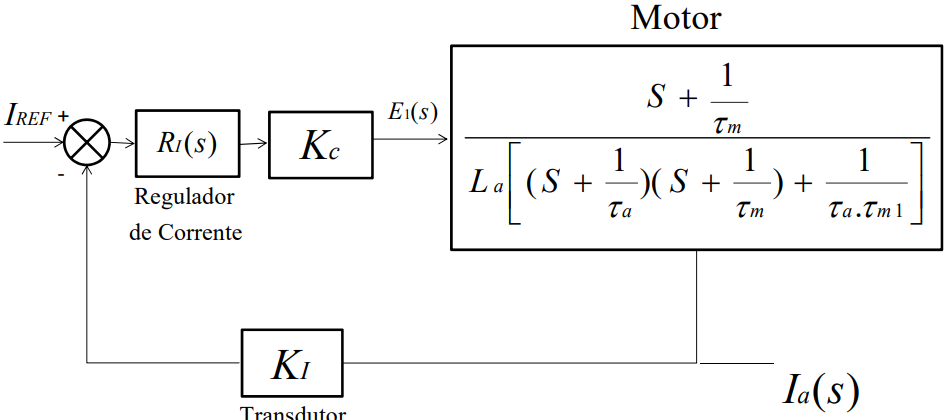
\includegraphics[scale= 0.55]{imagens/diagrama1_51.png}
\caption{\label{fig:D1_51} Malha de regulação de corrente.}
\caption*{Fonte: MARTINS, cap. 3, eslaide 2.}
\end{figure}

Sendo um regulador de corrente proporcional,

$R_{l}(s) = K_{l}; \tau_{l} = \frac{R_{a}J}{K_{e}K_{t}}$.

Para os estudos realizados a seguir considera-se que $\tau_{a} << \tau_{m}$, então $\tau_{a}$ pode ser desprezado em relação a $\tau_{m}$.

Dessa forma o modelo do motor é representado pela seguinte função:

\[\frac{I_{a}(s)}{E_{l}} = \frac{\left(\tau_{m}s + 1\right)}{\left(\frac{L_{a}}{\tau_{a}}\right)\left[\left(1 + s\tau_{a}\right)\left(1 + s\tau_{m}\right) + \left(\frac{\tau_{m}}{\tau_{ml}}\right)\right]}\]

Onde, $\frac{L_{a}}{\tau_{a}} = R_{a}$. Assim:

\[\frac{I_{a}(s)}{E_{l}} = \frac{\left(\tau_{m}s + 1\right)}{R_{a}\left[\left(1 + s\tau_{m}\right) + \left(\frac{\tau_{m}}{\tau_{ml}}\right)\right]}\]

\[1 +s\tau_{m} + \frac{\tau_{m}}{\tau_{ml}} = \tau_{m}\left(s + \frac{1}{\tau_{m}} +\frac{1}{\tau_{ml}}\right) = \tau_{m}\left[s + \frac{\left(\tau_{m} + \tau_{ml}\right)}{\tau_{m}\tau_{ml}}\right] = \frac{\tau_{m} + \tau_{ml}}{\tau_{ml}}\left(1 + s\frac{\tau_{m}\tau_{ml}}{\tau_{m} + \tau_{ml}}\right)\]

Seja $K_{1} = \frac{\tau_{m1}}{R_{a}\left(\tau_{m} + \tau_{m1}\right)} = \frac{D}{K_{e}^{2} + DR{a}}$ e $\tau_{m2} = \frac{\tau_{m}\tau_{m1}}{\tau_{m} + \tau_{m1}}$

Onde, $D = \frac{J}{\tau_{m}}$

Assim:
\[\frac{I_{a}(s)}{E_{1}(s)} = K_{1}\frac{\left(1 + s\tau_{m}\right)}{1 + s\tau_{m2}} \]

Dessa forma, o diagrama de blocos é representado pela figura \ref{fig:D2_51}.

\begin{figure}[ht!]
\center
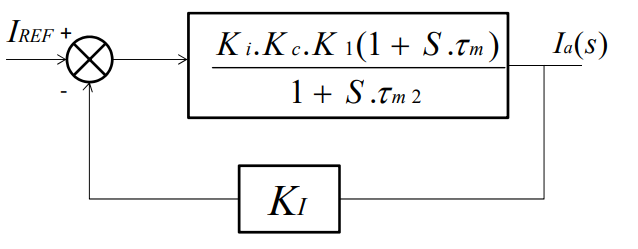
\includegraphics[scale= 0.55]{imagens/diagrama2_51.png}
\caption{\label{fig:D2_51} Diagrama de blocos do motor CC com regulador de corrente.}
\caption*{Fonte: MARTINS, cap. 3, eslaide 4.}
\end{figure}

Logo:
\[\frac{I_{a}(s)}{I_{REF}(s)} = \frac{K_{i}K_{e}K_{1}\frac{\left(1 + s\tau_{m}\right)}{1 + s\tau_{m2}}}{1 + K_{i}K_{c}K_{1}K_{I}\frac{1 + s\tau_{m}}{1 + s\tau_{m2}}}\]

Assim:
\[\frac{I_{a}(s)}{I_{REF}(s)} = \frac{K_{i}K_{c}K_{1}\left(1 + s\tau_{m}\right)}{\left(1 + s\tau_{m2}\right) + K_{i}K_{c}K_{1}\left(1 + s\tau_{m}\right)}\]

\[\frac{I_{a}(s)}{I_{REF}(s)} = \frac{K_{i}K_{c}K_{1}\left(1 + s\tau_{m}\right)}{\left(1 + K_{i}K_{c}K_{1}K_{1}\right) + \left[1 + s\left(\frac{\tau_{m2} + K_{i}K_{c}K_{1}K_{I}\tau_{m} }{1 + K_{i}K_{c}K_{1}K_{I}}\right)\right]}\]

Seja um $K_{i}$ escolhido de modo que $K_{i}.K_{c}.K_{1}.K_{I} >> 1$. Assim:

\[\frac{I_{a}(s)}{I_{REF}(s)} = \frac{K_{i}K_{c}K_{1}\left(1 + s\tau_{m}\right)}{ K_{i}K_{c}K_{1}\left(1 + s\tau_{m3}\right)}\]

Onde, $\tau_{m3} = \frac{\tau_{m2}}{K_{i}K_{c}K_{1}K_{I}} + \tau_{m}$

Um $K_{i}$ grande, além de diminuir o erro estático, torna $\tau_{m3} = \tau_{m}$ o que implica no cancelamento pólo-zero da malha. Assim:

\[\frac{I_{a}(s)}{I_{REF}(s)} \frac{1}{K_{I}}\]

Desse modo, para se limitar a corrente de armadura do motor, basta limitar a corrente de referência $I_{REF}(s)$. 

Dado que a equação a seguir define o erro estático relativo
\[\epsilon_{R} = \frac{I_{REF} - K_{I}I_{a}}{I_{REF}}  ,\]
é possível provar que:
\[K_{i} = \frac{1 - \epsilon_{R}}{\epsilon_{R}}K_{c}K_{1}K_{I}\]

\subsubsection{Malha de velocidade}

O diagrama de blocos ilustrado na figura \ref{fig:D1_53} representa a malha de velocidade.

\begin{figure}[ht!]
\center
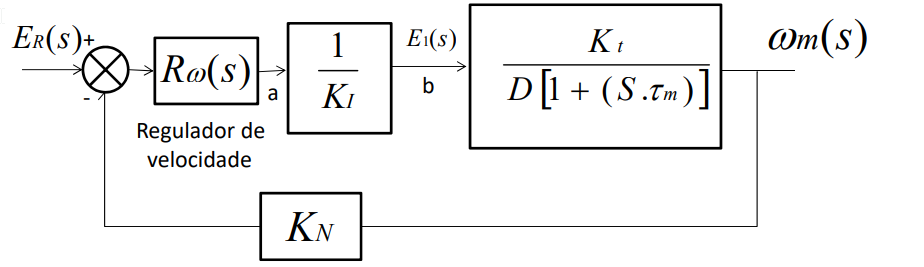
\includegraphics[scale= 0.55]{imagens/diagrama1_53.png}
\caption{\label{fig:D1_53} Diagrama de blocos para estudo da malha de velocidade.}
\caption*{Fonte: MARTINS, cap. 3, eslaide 7.}
\end{figure}

Onde, $D = \frac{J}{\tau_{m}}$
Seja um controlador proporcional integral para a velocidade. Assim:
\[R_{w}(s) = 	\left ( A + \dfrac{B}{s} \right ) = \frac{As + B}{s} = \frac{\left(1 + \frac{A}{B}s\right)}{\frac{s}{B}}\]

\[R_{w}(s) = A \frac{\left(1 + \frac{A}{B}s\right)}{\frac{A}{B}s} = \frac{A\left(1 + \tau_{c}s\right)}{s\tau_{c}}\]

Onde:
\[\tau_{c} = \frac{A}{B}\]

Portanto, a figura \ref{fig:D2_53} ilustra o diagrama de blocos conforme as equações anteriores.

\begin{figure}[ht!]
\center
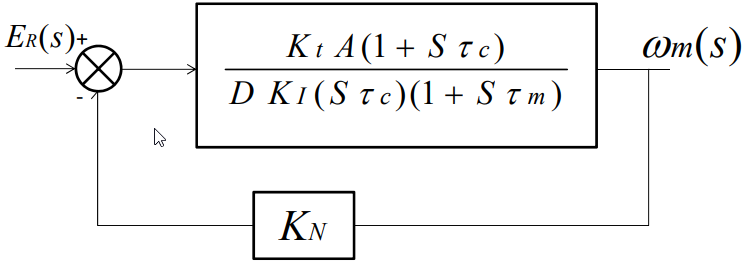
\includegraphics[scale= 0.55]{imagens/diagrama2_53.png}
\caption{\label{fig:D2_53} Estudo da malha de velocidade usando regulador proporcional-integral.}
\caption*{Fonte: MARTINS, cap. 3, eslaide 8.}
\end{figure}

Portanto:

\[\frac{\omega_{m}(s)}{E_{R}(s) } =  \frac{\left(\frac{K_{t}A}{DK_{I}}\frac{\left(1 + \tau_{c}s\right)}{s\tau_{C}\left(1 + s\tau_{m}\right)}\right)}{\left[1 + \left(\frac{K_{t}AK_{N}}{DK_{I}}\frac{\left(1 + \tau_{c}s\right)}{s\tau_{c}\left(1 + s\tau_{m}\right)}\right)\right]}\]

Assim:
 
\[\frac{\omega_{m}(s)}{E_{R}(s) } = \frac{K_{t}A\left(1 + s\tau_{c}\right)}{DK_{t}s\tau_{c}\left(1 + s\tau_{M} + K_{t}AK_{N}\left(1 + s\tau_{c}\right)\right)}\]

\[\frac{\omega_{m}(s)}{E_{R}(s) } = \frac{\frac{1 + s\tau_{c}}{K_{N}}}{1 + \tau_{c}\left(1 + \frac{DK_{I}}{K_{t}K_{N}A}\right)s + \frac{DK_{I}\tau_{c}\tau_{m}}{K_{t}AK_{N}}s^{2} }\]

Seja:
\[\frac{K_{t}AK_{N}}{K} >> 1\]

Portanto:
\[\frac{\omega_{m}(s)}{E_{R}(s) } = \frac{\left(1 + s\tau_{c}/K_{N}\right)}{1 + s\tau_{c} + s^{2}\tau_{c}\tau_{2}}\]

\[ \tau_{2} = \frac{DK_{I}\tau_{m}}{K_{t}K_{N}A}\]

Os pólos da função de transferência são obtidos do seguinte modo:

\[1 + s\tau_{c} + \tau_{c}\tau_{2}s^{2} = 0\]

\[ s^{2} + \frac{1}{\tau_{2}}s + \frac{1}{\tau_{2}\tau_{c}} = 0\]

\[s_{1},s_{2} = \frac{\frac{-1}{\tau_{2}} \pm \sqrt{\frac{1}{\tau_{2}^{2}} - \frac{4}{\tau_{2}\tau_{c}}}}{2}\]

Desta forma:

\[s_{1},s_{2} = \frac{-1}{2\tau_{2}} \pm j\frac{1}{2}\sqrt{\frac{4}{\tau_{2}\tau_{c}}}\sqrt{1 - \frac{\tau_{c}}{4\tau_{2}}}\]

\[s_{1},s_{2} = -\epsilon\omega_{n} \pm j\omega_{n}\sqrt{1 - \epsilon^{2}}\]

Dado que :

$\omega_{n}$ =  Frequência natural não amortecida

$\epsilon$ = Fator de amortecimento relativo


Na prática: $\epsilon = 0,707$
Portanto:
\[\tau_{c} = 2\tau_{2}\]
\[\omega_{n} = \frac{1}{\tau_{2}\sqrt{2}}\]

Escolhendo-se $\omega_{n}$ pode-se obter $\tau_{2}$ e $\tau_{c}$. Sabendo o valor de $\tau_{2}$, pode-se obter A com a seguinte expressão:

\[A = \frac{DK_{I}\tau_{m}}{K_{I}K_{N}\tau_{2}} = \frac{K_{I}J}{K_{t}K_{N}\tau_{2}}\]

Dessa forma os parâmetros do regulador $P_{I}$ podem ser determinados.

Exemplo de cálculo:

Seja um motor CC de 3 HP, 125 V, 1750 rpm, com os seguintes valores:

$R_{a} = 0,6 \Omega$ 

$L_{a} = 0,006 H$

$J = 0,093 Kgm^{2}$ (máquina mais carga)

$D = 0,008 Nm/rad/s$

$K_{t} = K_{c} = 0,6 V/rad/s$

É adicionado externamente um indutor com os seguintes parâmetros:

$L_{ext} = 0,04H$
$R_{ext} = 0,4\Omega$

Desse modo, aplicando-se as equações já desenvolvidas no estudo teórico feito anteriormente obtém-se:

\[\tau_{a} = \frac{L_{a}}{R_{a}} = \frac{0,04 + 0,006}{0,4 + 0,6} = 0,046 seg\]
\[\tau = \frac{J}{D} = \frac{0,093}{0,008} = 11,63 seg\]

Os dados adicionais do problema são apresentados a seguir:

$K_{N} = 0,57 V/rad/s  \rightarrow $ Sensor de velocidade (tacogerador)

$K_{t} = 0,5 V/A  \rightarrow$ Transdutor de corrente.

$K_{C} = 25  \rightarrow$ Ganho do conversor.

Logo, tem-se que:

\[I_{a} = \frac{3.746}{125} = 18A\]
\[\frac{I_{a}}{I_{REF}} = \frac{1}{K_{I}} \rightarrow I_{REF} = 0,5.18 = 9 V \]

Seja $\omega_{n} = 10 rad/seg$ (frequência natural não amortecida). Então:
\[\tau_{2} \frac{1}{\omega_{n}\sqrt{2}}\]
\[\tau_{c} = 2\tau_{2}\]
\[\tau_{2} 0,07 seg\]
\[\tau_{c} = 0,14 seg\]

\[A = \frac{K_{I}J}{K_{t}K_{N}\tau_{2}} = \frac{0,5.0,093}{0,6.0,57.0,07} = 1,94\]
\[\tau_{c} = \frac{A}{B}\]

\[B = \frac{A}{\tau_{c}} = \frac{1,94}{0,14} = 13,86 \]

